\chapter{Materiales y Métodos}
\section{Materiales}
Para la evaluación y validación de los métodos de metrología de vista única desarrollados en este trabajo,
se ha empleado un conjunto de datos privado, capturado específicamente con fines experimentales.
Dicho conjunto fue recogido en diversas localizaciones del entorno urbano mediante un sistema multicámara,
en el que se estableció como referencia principal una cámara con sensor de profundidad. A continuación,
se describen las cámaras utilizadas, así como su disposición relativa y características técnicas.
\subsection{Sistema de captura}
\begin{table}[htp]
\scriptsize
\centering
\begin{tabular}{lcccc}
\hline
\textbf{Cámara} & \textbf{Tipo} & \textbf{Focal (mm)} & \textbf{CMOS} \\
\hline
RealSense D455 (RS) & Profundidad & 1.93 &  1/4'' OV9782 \\
Tapo C120 (Cam1) & Tipo cajero & 3.17 &  1/2.9'' \\
Dahua IPC-HDBW2831 (Cam2) & Domo & 2.8 &  1/2.7'' \\
Hikvision DS-2CD2046 (Cam3) & Bullet & 2.8 &  1/3'' \\
\hline
\end{tabular}
\caption{Características técnicas de las cámaras utilizadas}
\label{tab:CaptureSystem}
\end{table}
En la Tabla~\ref{tab:CaptureSystem} se recogen las características técnicas de cada una de las cámaras.
Cada una de ellas se monta en su respectivo tripod. Se utiliza la cámara ``Intel RealSense D455'' (RS) como principal y
se calcula el posicionamiento de las demás en términos relativos (véase información adicional en el Apéndice~\ref{app:LocationConfig}).
Esto es debido a que se utilizará el sensor de profundidad, ``CMOS 1/4'' OV9782'', de la cámara RS para realizar los cálculos necesarios para estimar el
tamaño de los objetos en escena utilizando el método clásico. Las cámaras empiezan a grabar simúltaneamente, almacenando
la información tanto en memoria como a través de la red. Se obtienen grabaciones en cuatro ubicaciones diferentes: una sala de seminarios,
una rampa de entrada, un aparcamiento y una acera (véase la Figura~\ref{fig:DataExamples}).
\begin{figure}[htp]
\begin{center}
    \subfloat{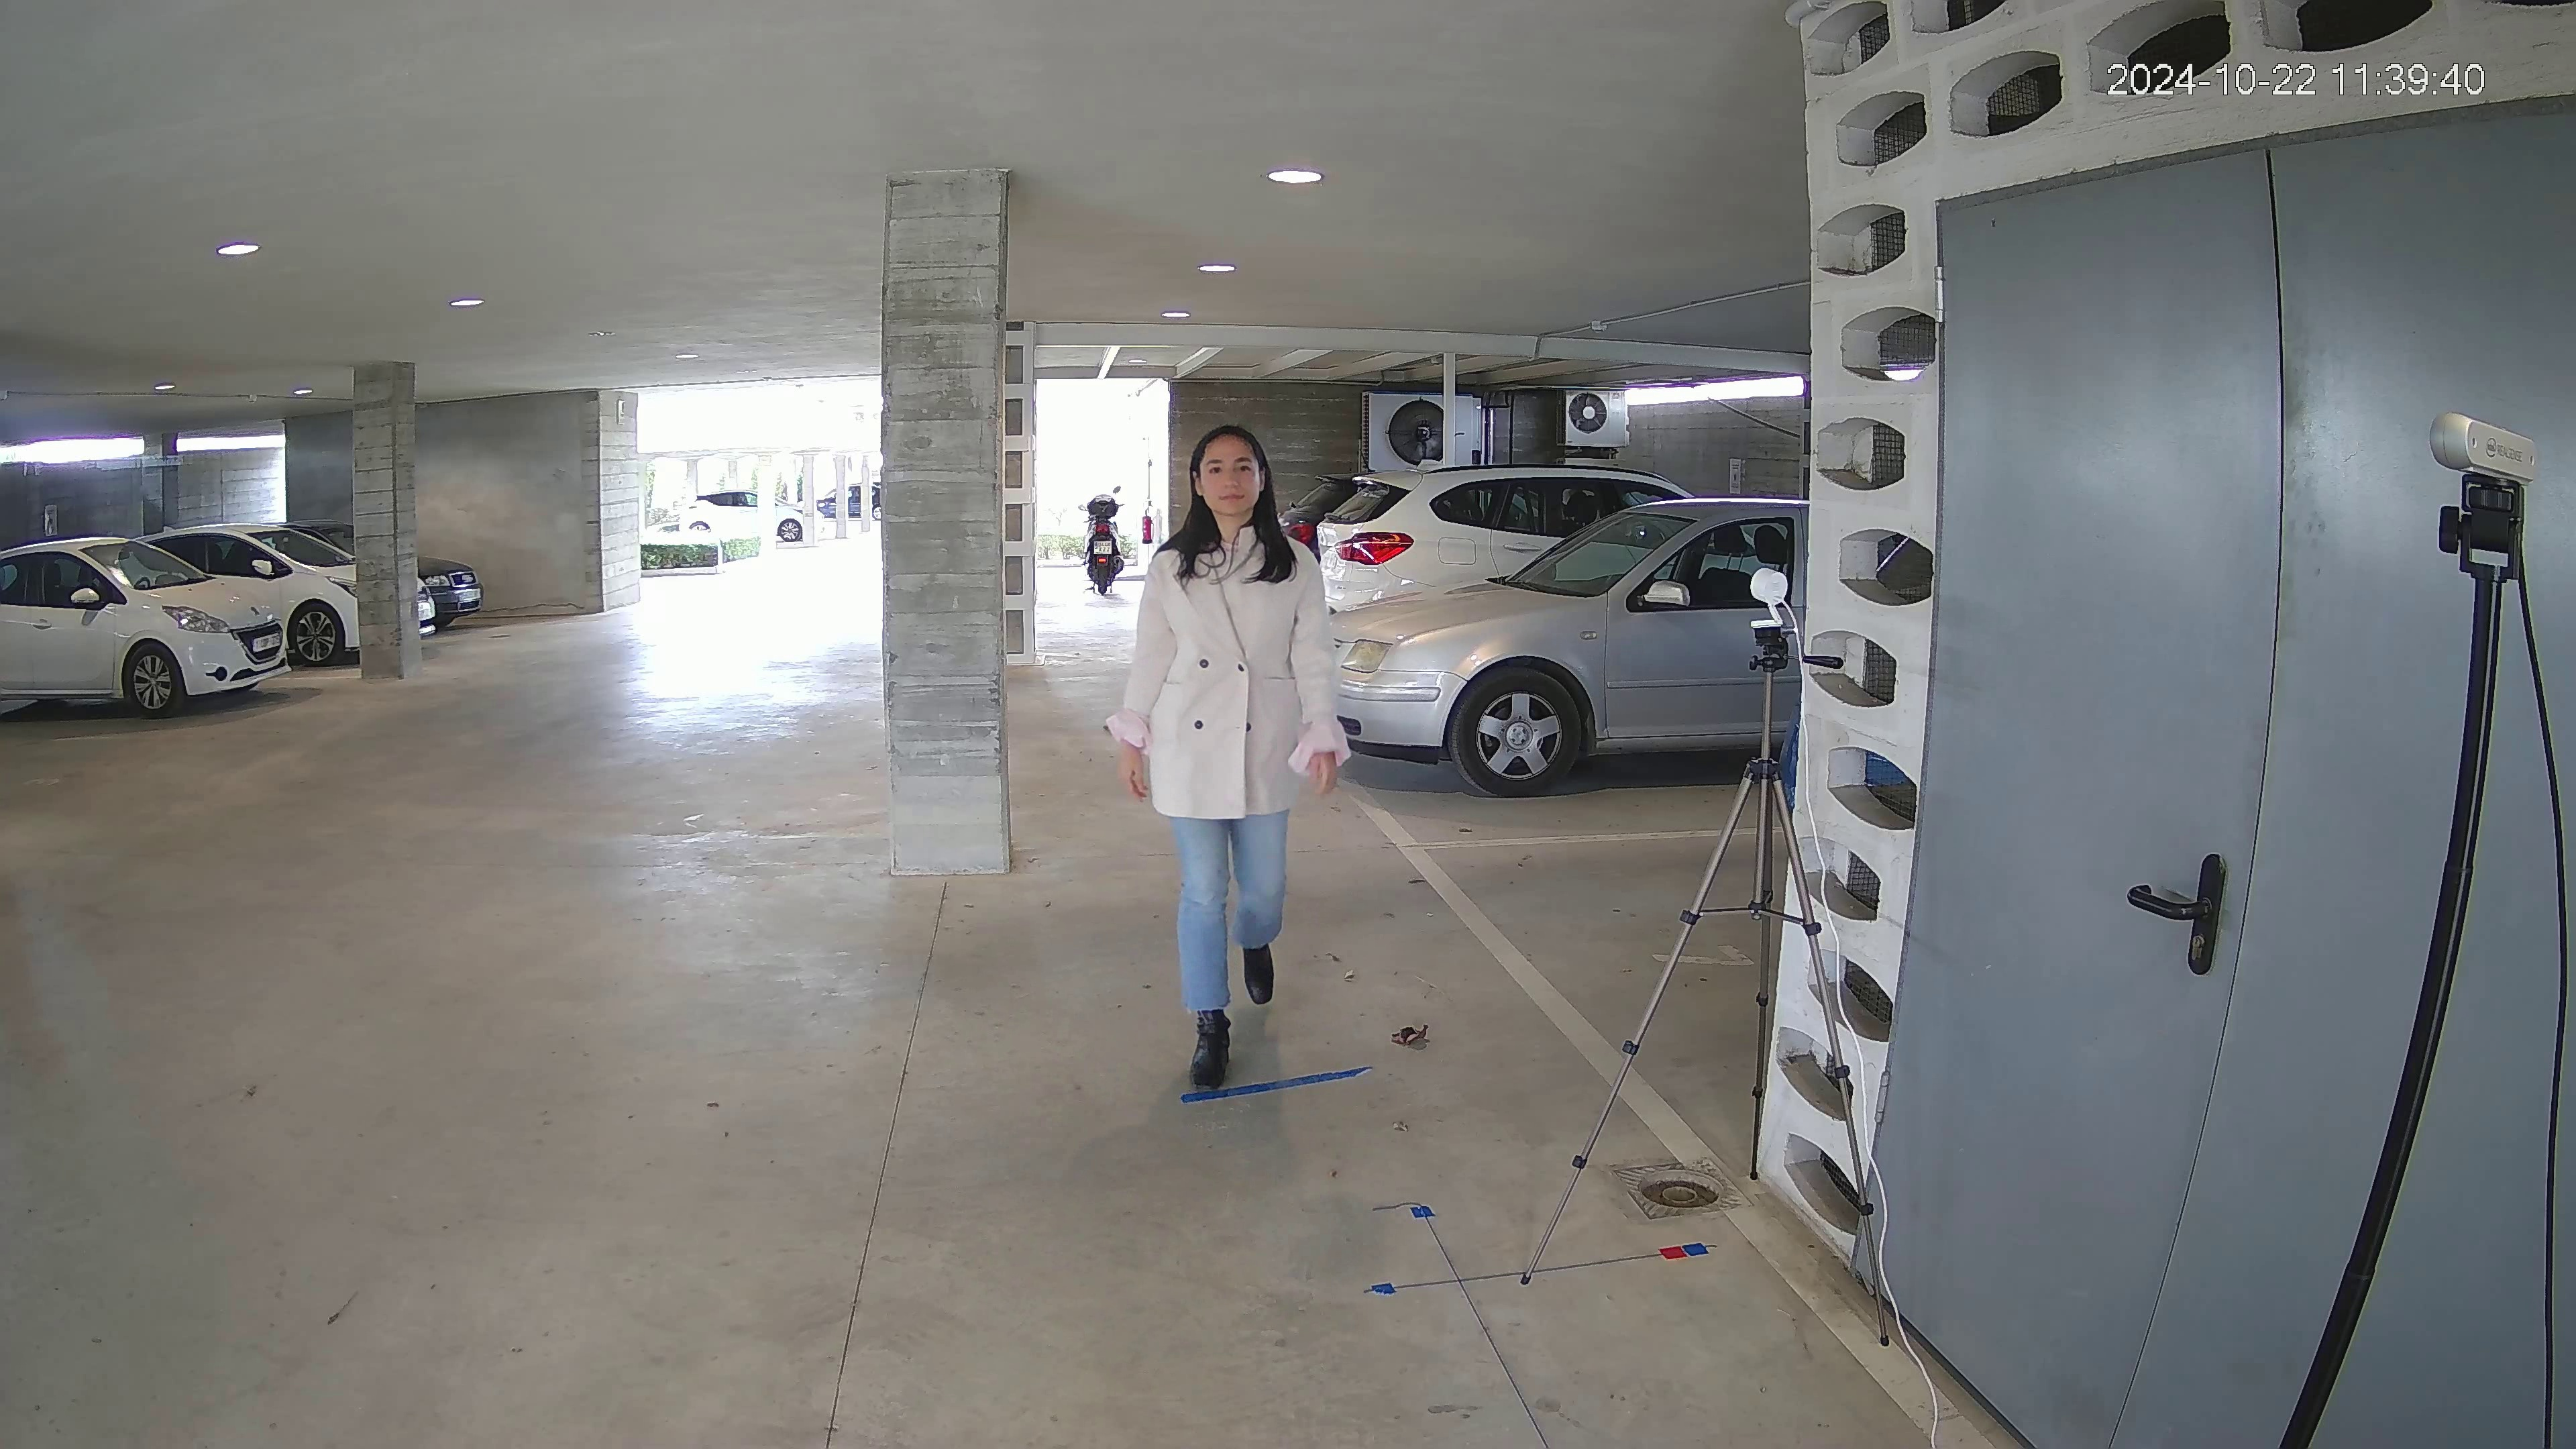
\includegraphics[width=0.5\textwidth]{imagenes/chapter4/ParkingLot.jpg}}
    \subfloat{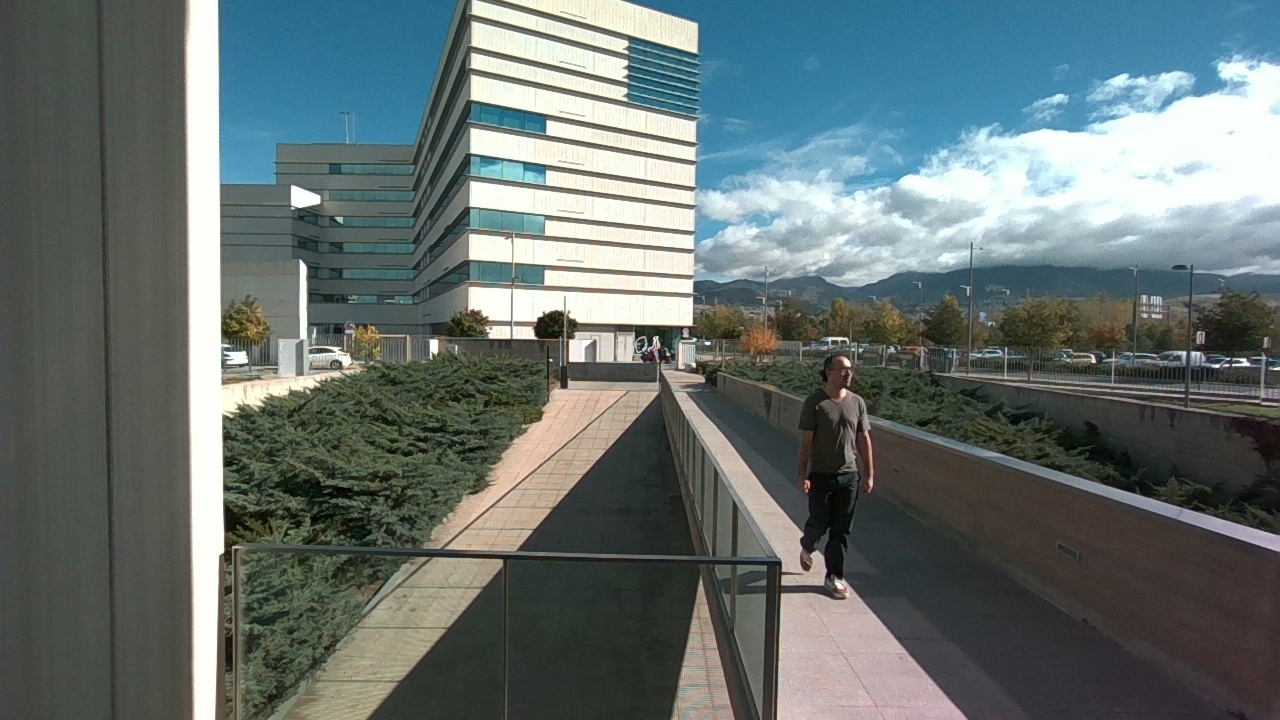
\includegraphics[width=0.5\textwidth]{imagenes/chapter4/EntranceRamp.jpg}}\\
    \subfloat{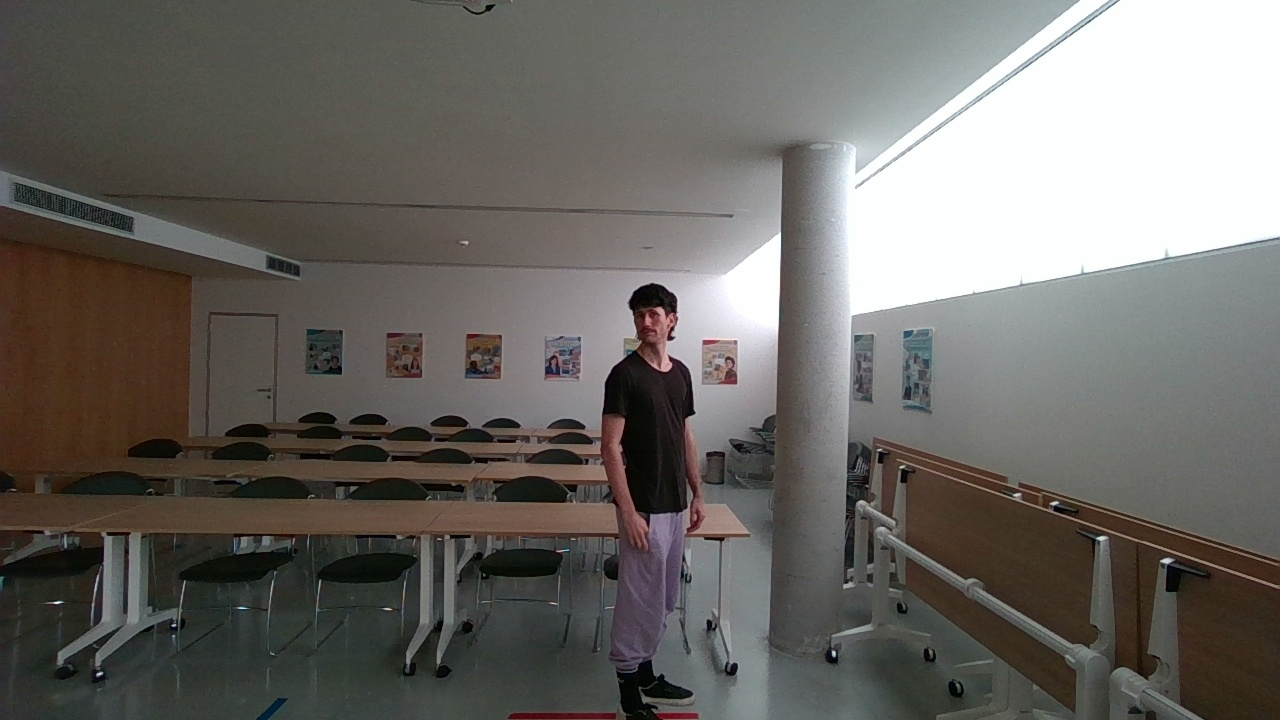
\includegraphics[width=0.5\textwidth]{imagenes/chapter4/SeminarRoom.jpg}}
    \subfloat{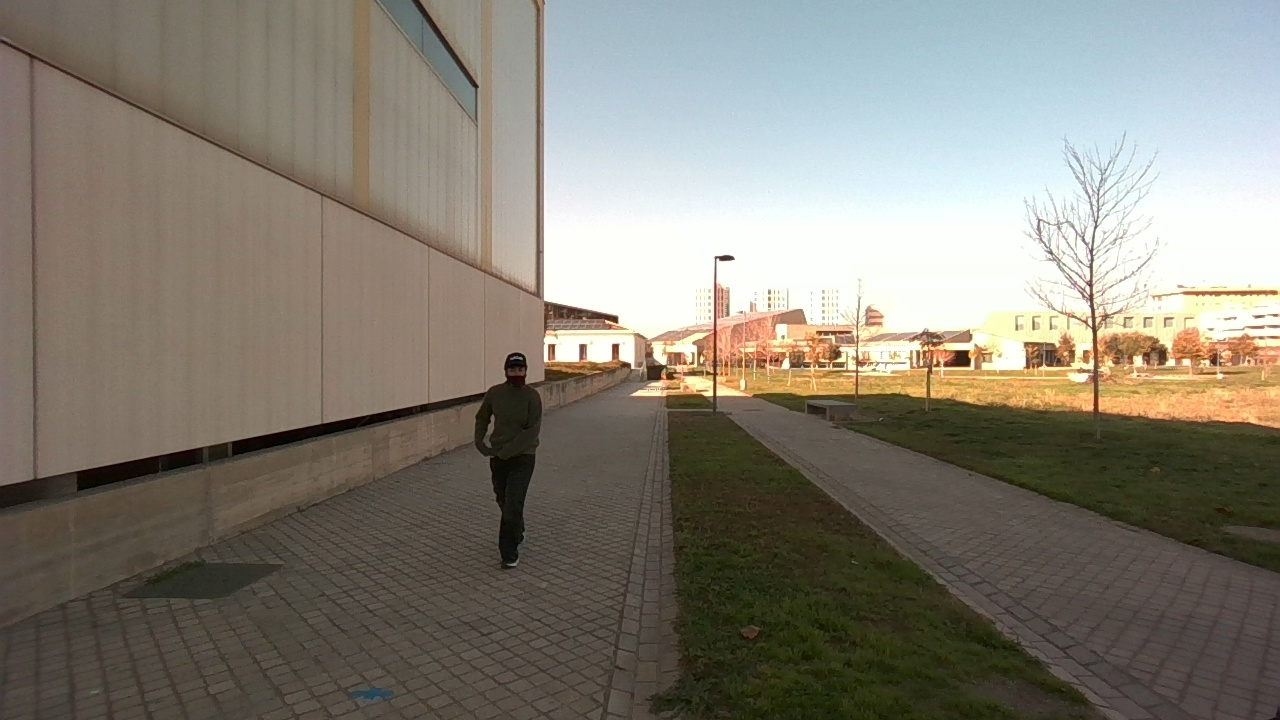
\includegraphics[width=0.5\textwidth]{imagenes/chapter4/Sidewalk.jpg}}
\end{center}
\caption{Ejemplo de grabaciones realizadas en las diferentes ubicaciones.}
\label{fig:DataExamples}
\end{figure}

% Nice end phrase perhaps?
Este conjunto de datos, capturado bajo condiciones reales y desde múltiples puntos de vista, ha permitido una evaluación robusta de
los métodos propuestos, facilitando el análisis de su rendimiento frente a diferentes configuraciones geométricas y
tipos de cámaras de vigilancia.
\section{Métodos}
